\documentclass[12pt, titlepage]{article}
\usepackage{graphicx}
\usepackage{booktabs}
\usepackage{tabularx}
\usepackage{float}
\usepackage{hyperref}
\hypersetup{
    colorlinks,
    citecolor=black,
    filecolor=black,
    linkcolor=red,
    urlcolor=blue
}
\usepackage[round]{natbib}

\usepackage{color}

\newif\ifcomments\commentstrue

\ifcomments
\newcommand{\authornote}[3]{\textcolor{#1}{[#3 ---#2]}}
\newcommand{\todo}[1]{\textcolor{red}{[TODO: #1]}}
\else
\newcommand{\authornote}[3]{}
\newcommand{\todo}[1]{}
\fi

\newcommand{\wss}[1]{\authornote{blue}{SS}{#1}} 
\newcommand{\plt}[1]{\authornote{magenta}{TPLT}{#1}} %For explanation of the template
\newcommand{\an}[1]{\authornote{cyan}{Author}{#1}}


\begin{document}

\title{Test Report: Stoichiometry Mass-Mass Program} 
\author{Deema Alomair}
\date{\today}
	
\maketitle

\pagenumbering{roman}

\section{Revision History}

\begin{tabularx}{\textwidth}{p{3cm}p{2cm}X}
\toprule {\bf Date} & {\bf Version} & {\bf Notes}\\
\midrule
26/12/2019 & 1.0 & First version of the document\\
\bottomrule
\end{tabularx}

~\newpage

\section{Symbols, Abbreviations and Acronyms}

\renewcommand{\arraystretch}{1.2}
\begin{tabular}{l l} 
  \toprule		
  \textbf{symbol} & \textbf{description}\\
  \midrule 
  T & Test\\
  SMMP & Stoichiometry Mass-Mass Program\\
  \bottomrule
\end{tabular}\\

\newpage

\tableofcontents

\listoftables 

\listoffigures


\newpage

\pagenumbering{arabic}

This document report result from unit test cases found in Unit  Verification and Validation Plan document \cite{UnitVnVPlan}.

\section{Functional Requirements Evaluation}

Functional requirement is evaluated using unit test cases from T1 to T17. All the details regarding functional requirements evaluation can be found in section~\ref{unit}. The traceability between unit test cases and functional requirement found in table ~\ref{Table:R_trace} of section ~\ref{functional}.

\section{Nonfunctional Requirements Evaluation}
Nonfunctional Requirements Evaluated in unit test cases T18 - T19. All the details regarding Nonfunctional requirements evaluation can be found in this section. The traceability between unit test cases and Nonfunctional requirement found in table ~\ref{Table:R_trace1} of section ~\ref{functional}.

\subsection{Usability}

Unit test T18 measures the Usability of SMMP system. The survey measured the satisfaction level of potential user after using SMMP. How easy and understandable the system is?. It needs to be filled by any user and if satisfactory level is low then enhancement need to be taken into account. 

\subsection{Reliability}

Unit test T19 measures the Reliability of SMMP system. 25 different unbalanced chemical reactions were tested and compared to answer of online balancer \cite{OnlineBalancer} as parallel testing. the aim was to get 100\% of correct answers that includes right balance reaction and correct mass value. Below table shows the final result compared to the online balancer and the final percentage of correctness 

\begin{table}[h!]
\centering
\resizebox{\textwidth}{!}{\begin{tabular}{|c|c|c|c|}
\hline
 Unbalanced Chemical Reaction & Online Balancer Result & SMMP Result  & correctness \\
\hline
C$H_4$ + $O_2$ $\rightarrow$ C$O_2$ + $H_2$O  & C$H_4$ + 2$O_2$ $\rightarrow$ C$O_2$ + 2$H_2$O  & C$H_4$ + 2$O_2$ $\rightarrow$ C$O_2$ + 2$H_2$O  &  correct  \\ \hline
$Fe_2$$O_3$ + C $\rightarrow$ Fe + C$O_2$  & 2$Fe_2$$O_3$ + 3C $\rightarrow$ 4Fe + 3C$O_2$ & 2$Fe_2$$O_3$ + 3C $\rightarrow$ 4Fe + 3C$O_2$ & correct   \\ \hline
$N_2$ + $O_2$ $\rightarrow$ $N_2$$O_5$ & 2$N_2$ + 5$O_2$ $\rightarrow$ 2$N_2$$O_5$ & 2$N_2$ + 5$O_2$ $\rightarrow$ 2$N_2$$O_5$& correct  \\ \hline
C$H_4$ + $Cl_2$ $\rightarrow$  C$Cl_4$ + HCl & C$H_4$ + 4$Cl_2$ $\rightarrow$  C$Cl_4$ + 4HCl & 4C$H_4$ + $Cl_2$ $\rightarrow$  C$Cl_4$ + 4HCl & correct   \\ \hline
$N_2$ + $H_2$ $\rightarrow$ $NH_3$ & $N_2$ + 3$H_2$ $\rightarrow$ 2$NH_3$ & $N_2$ + 3$H_2$ $\rightarrow$ 2$NH_3$ & correct \\ \hline
Fe + $H_2$O $\rightarrow$ $Fe_3$$O_4$ + $H_2$ & 3Fe + 4$H_2$O $\rightarrow$ $Fe_3$$O_4$ + 4$H_2$ & 3Fe + 4$H_2$O $\rightarrow$ $Fe_3$$O_4$ + 4$H_2$ & correct \\ \hline
Xe + $F_2$ $\rightarrow$ Xe$F_6$ & Xe + 3$F_2$ $\rightarrow$ Xe$F_6$ & Xe + 3$F_2$ $\rightarrow$ Xe$F_6$ & correct  \\ \hline
Hg + $O_2$ $\rightarrow$ HgO & 2Hg + $O_2$ $\rightarrow$ 2HgO & 2Hg + $O_2$ $\rightarrow$ 2HgO & correct  \\ \hline
CaO + C $\rightarrow$ Ca$C_2$ + CO & CaO + 3C $\rightarrow$ Ca$C_2$ + CO & CaO + 3C $\rightarrow$ Ca$C_2$ + CO & correct  \\ \hline
$S_8$ + $F_2$ $\rightarrow$ $SF_6$ & $S_8$ + 24$F_2$ $\rightarrow$ 8$SF_6$ & $S_8$ + 24$F_2$ $\rightarrow$ 8$SF_6$ & correct  \\ \hline
Mg + $N_2$ $\rightarrow$ $Mg_3$$N_2$ & 3Mg + $N_2$ $\rightarrow$ $Mg_3$$N_2$ & 3Mg + $N_2$ $\rightarrow$ $Mg_3$$N_2$ & correct  \\ \hline
Be$F_2$ + Mg $\rightarrow$ Mg$F_2$ + Be & balance & balance & correct  \\ \hline
Zn + HCl $\rightarrow$ Zn$Cl_2$ + $H_2$ & Zn + 2HCl $\rightarrow$ Zn$Cl_2$ + $H_2$ & Zn + 2HCl $\rightarrow$ Zn$Cl_2$ + $H_2$ & correct  \\ \hline
SiC + $Cl_2$ $\rightarrow$ Si$Cl_4$ + C & SiC + 2$Cl_2$ $\rightarrow$ Si$Cl_4$ + C & SiC + 2$Cl_2$ $\rightarrow$ Si$Cl_4$ + C & correct \\ \hline
MnS + HCl $\rightarrow$ $H_2$S + Mn$Cl_2$ & MnS + 2HCl $\rightarrow$ $H_2$S + Mn$Cl_2$ & MnS + 2HCl $\rightarrow$ $H_2$S + Mn$Cl_2$ & correct  \\ \hline
 U$F_4$ + Mg $\rightarrow$ Mg$F_2$ + U & U$F_4$ + 2Mg $\rightarrow$ 2Mg$F_2$ + U &  U$F_4$ + 2Mg $\rightarrow$ 2Mg$F_2$ + U & correct  \\ \hline
S + $N_2$O $\rightarrow$ S$O_2$ + $N_2$ & S + 2$N_2$O $\rightarrow$ S$O_2$ + 2$N_2$ & S + 2$N_2$O $\rightarrow$ S$O_2$ + 2$N_2$ & correct  \\ \hline
Si$H_4$ + $O_2$ $\rightarrow$ Si$O_2$ + $H_2$O & Si$H_4$ + 2$O_2$ $\rightarrow$ Si$O_2$ + 2$H_2$O & Si$H_4$ + 2$O_2$ $\rightarrow$ Si$O_2$ + 2$H_2$O & correct  \\ \hline
Ti$Cl_4$ + Mg $\rightarrow$ Mg$Cl_2$ + Ti & Ti$Cl_4$ + 2Mg $\rightarrow$ 2Mg$Cl_2$ + Ti  & Ti$Cl_4$ + 2Mg $\rightarrow$ 2Mg$Cl_2$ + Ti & correct  \\ \hline
Si + $S_8$ $\rightarrow$ $Si_2$$S_4$ & 4Si + $S_8$ $\rightarrow$ 2$Si_2$$S_4$ & 4Si + $S_8$ $\rightarrow$ 2$Si_2$$S_4$ & correct \\ \hline
Si$O_2$ + HF $\rightarrow$ Si$F_4$ + $H_2$O & Si$O_2$ + 4HF $\rightarrow$ Si$F_4$ + 2$H_2$O & Si$O_2$ + 4HF $\rightarrow$ Si$F_4$ + 2$H_2$O & correct \\ \hline
$P_4$ + $O_2$ $\rightarrow$ $P_2$$O_5$ & $P_4$ + 5$O_2$ $\rightarrow$ 2$P_2$$O_5$ & $P_4$ + 5$O_2$ $\rightarrow$ 2$P_2$$O_5$& correct \\ \hline
Sb + $O_2$ $\rightarrow$ $Sb_4$$O_6$ & 4Sb + 3$O_2$ $\rightarrow$ $Sb_4$$O_6$ & 4Sb + 3$O_2$ $\rightarrow$ $Sb_4$$O_6$ & correct \\ \hline
U$O_2$ + HF $\rightarrow$ U$F_4$ + $H_2$O  & U$O_2$ + 4HF $\rightarrow$ U$F_4$ + 2$H_2$O  & U$O_2$ + 4HF $\rightarrow$ U$F_4$ + 2$H_2$O & correct \\ \hline
Al + $O_2$ $\rightarrow$ $Al_2$$O_3$ & 4Al + 3$O_2$ $\rightarrow$ 2$Al_2$$O_3$ & 4Al + 3$O_2$ $\rightarrow$ 2$Al_2$$O_3$ & correct  \\ \hline
\hline
\end{tabular}}
\caption{Reliability testing of SMMP as comparison to online balancer.}
\label{Table:R_trace}
\end{table}

The goal of Reliability had been accomplished. all tested reactions were balanced correctly as compared to the online balancer. 
	
\section{Comparison to Existing Implementation}	

This is stand alone system. If there is any existing systems with same functionalities and goals the developer is not aware about them and no comparison had  been made. 

\section{Unit Testing}\label{unit}

\subsection{T1: get number of chemical reaction elements}

The goal of this test is to make sure that at least one element for reactant1 , reactant2 and product1 were entered by the user. this test is to fulfill the minimum requirements of balancing reaction with two reactant and one product. If user enter less than this requirement , an error massage should be shown. pictures below illustrates all possible entries by user that matches all cases of T1 ,Table1 in \cite{UnitVnVPlan}. The tests had been passed correctly and system responded as intended. 

\begin{figure}[h!]
 \begin{center}
 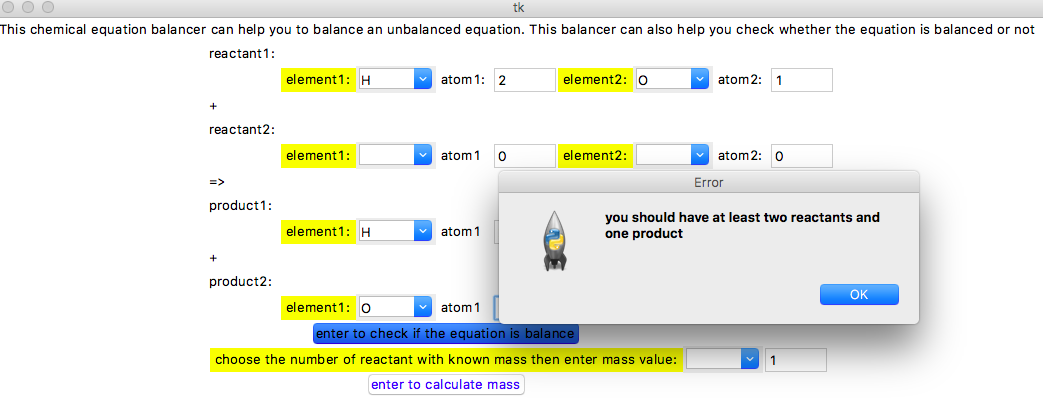
\includegraphics [width=\textwidth]{ElementNumber1}
 \caption{\label{ Figure 1:} error massage if user enter only one reactant}
 \end{center}
 \end{figure}
 
 \begin{figure}[h!]
 \begin{center}
 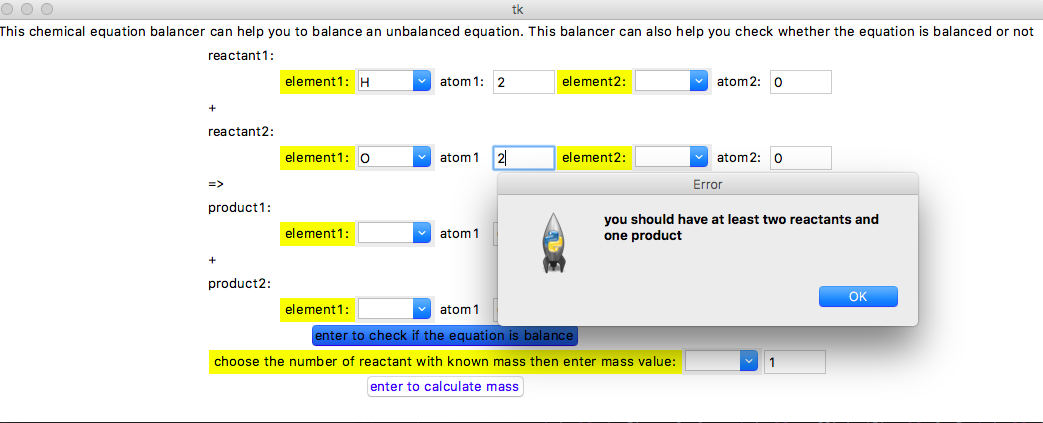
\includegraphics [width=\textwidth]{ElementNumber2}
 \caption{\label{ Figure 2:} error massage if user did not enter at least one product}
 \end{center}
 \end{figure}
 
 \begin{figure}[h!]
 \begin{center}
 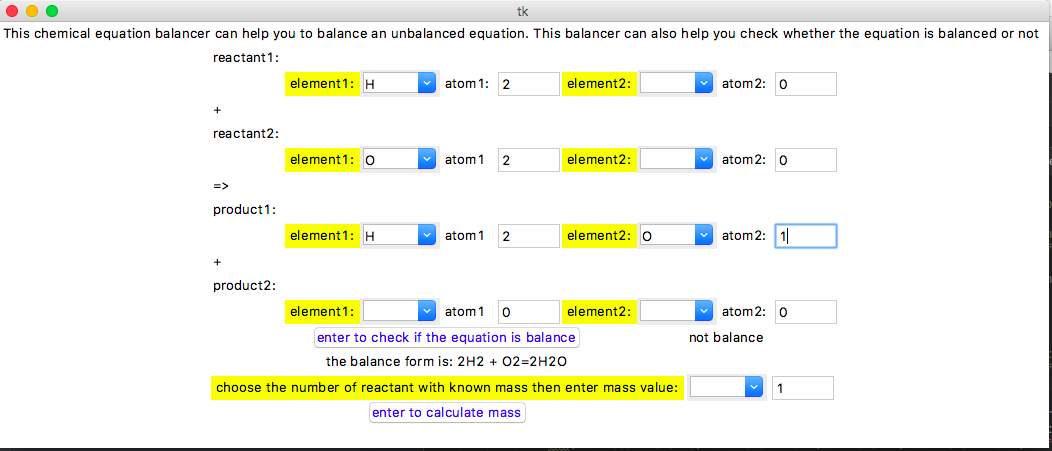
\includegraphics [width=\textwidth]{ElementNumber3}
 \caption{\label{ Figure 3:} system works fine with two reactants one product}
 \end{center}
 \end{figure}
 
 \begin{figure}[h!]
 \begin{center}
 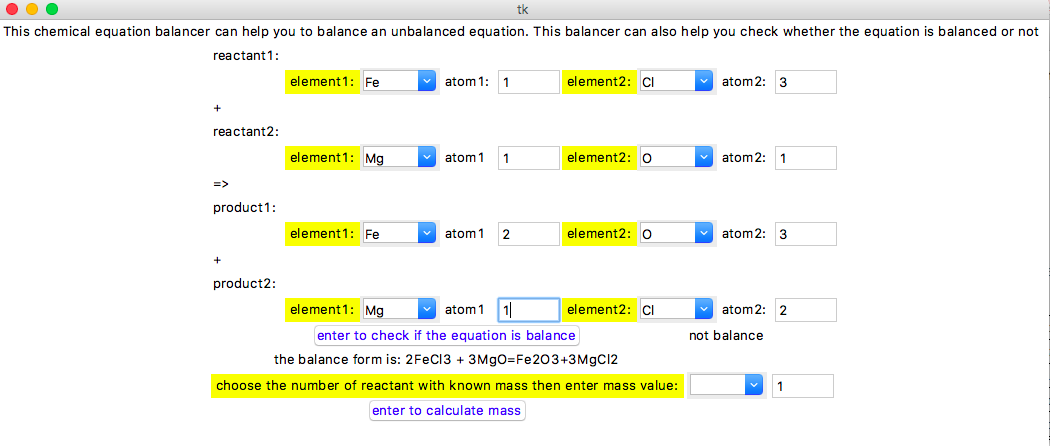
\includegraphics [width=\textwidth]{ElementNumber4}
 \caption{\label{ Figure 4:} system works fine with two reactants two product}
 \end{center}
 \end{figure}
 
\subsection{T2: get name of chemical reaction elements}

The goal of this test is to make sure that any chemical element involved in the reaction need to be in both sides, reactants and products sides. Every element enter the reaction must be also one of products. Failing to fulfill this requirement will cause an error massage. pictures below illustrates all possible entries by user that will rise an error massage which matches cases of T2 ,Table2 in \cite{UnitVnVPlan}. The tests had been passed correctly and system responded as intended. 

\begin{figure}[h!]
 \begin{center}
 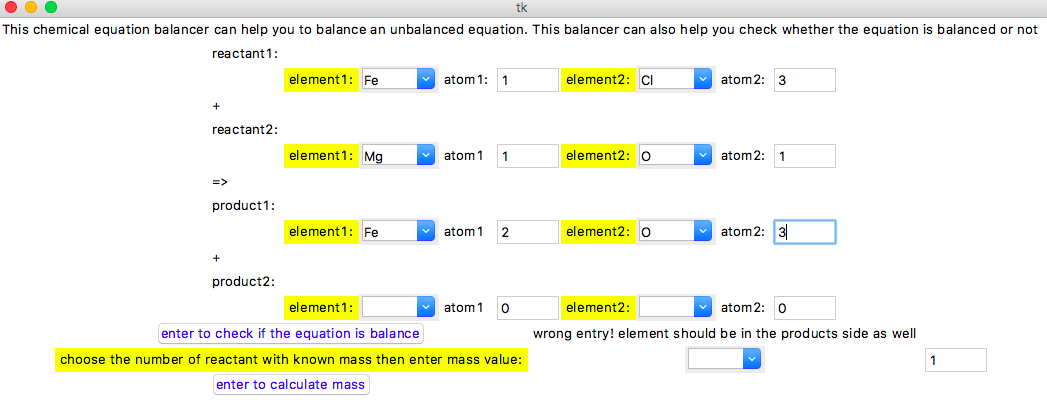
\includegraphics [width=\textwidth]{elementnameP}
 \caption{\label{ Figure 5:} error massage if user enter element only in reactant side}
 \end{center}
 \end{figure}
 
 \begin{figure}[h!]
 \begin{center}
 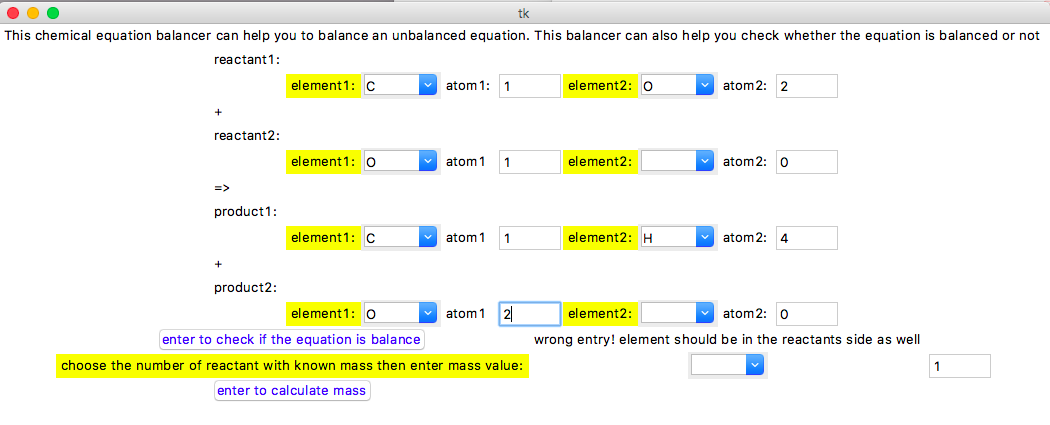
\includegraphics [width=\textwidth]{elementnameR}
 \caption{\label{ Figure 6:} error massage if user enter element only in product side}
 \end{center}
 \end{figure}
 
\subsection{T3: get atom value of chemical reaction elements}

The goal of this test is to make sure user change the default value of atom from 0 if he chose an element and enter a number greater than 0. pictures below illustrates all possible entries by user that cause error massage which matches cases of T3 ,Table3 in \cite{UnitVnVPlan}. The tests had been passed correctly and system responded as intended. 

\begin{figure}[h!]
 \begin{center}
 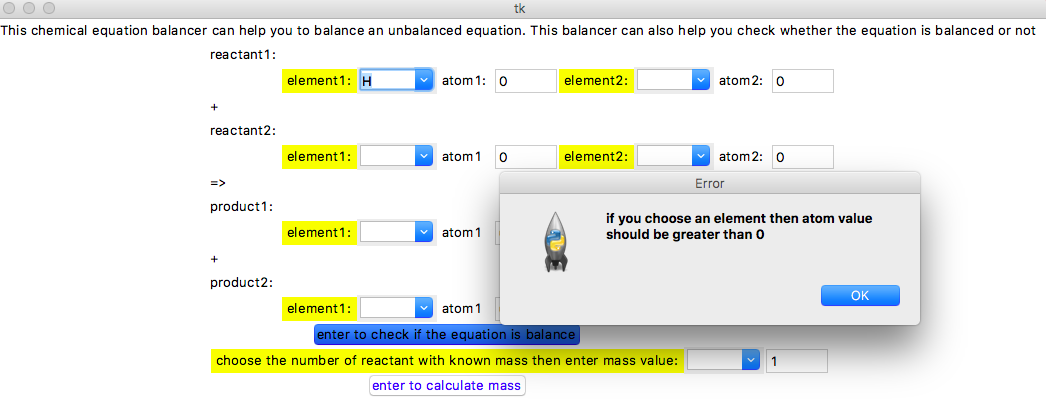
\includegraphics [width=\textwidth]{atomnegative}
 \caption{\label{ Figure 7:} error massage if user enter atom less than 1 if he selected an element}
 \end{center}
 \end{figure}
 
 \begin{figure}[h!]
 \begin{center}
 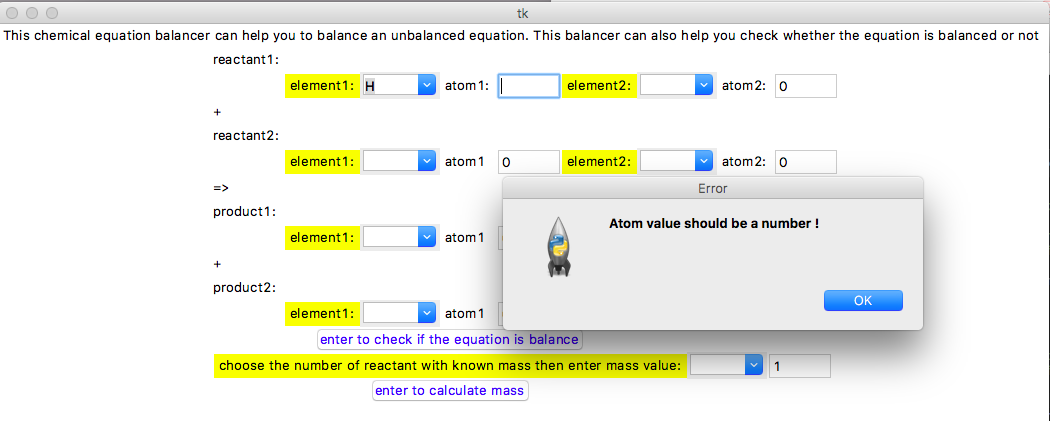
\includegraphics [width=\textwidth]{atomnotnumber}
 \caption{\label{ Figure 8:} error massage if user enter non number atom value}
 \end{center}
 \end{figure}
 
 
\subsection{T4: get Mass Input}

The goal of this test is to make sure user enter a positive number in mass value widget. the default mass value is 1. pictures below illustrates all possible entries by user that cause error massage which matches cases of T4 ,Table4 in \cite{UnitVnVPlan}. The tests had been passed correctly and system responded as intended. 

 \begin{figure}[H]
 \begin{center}
 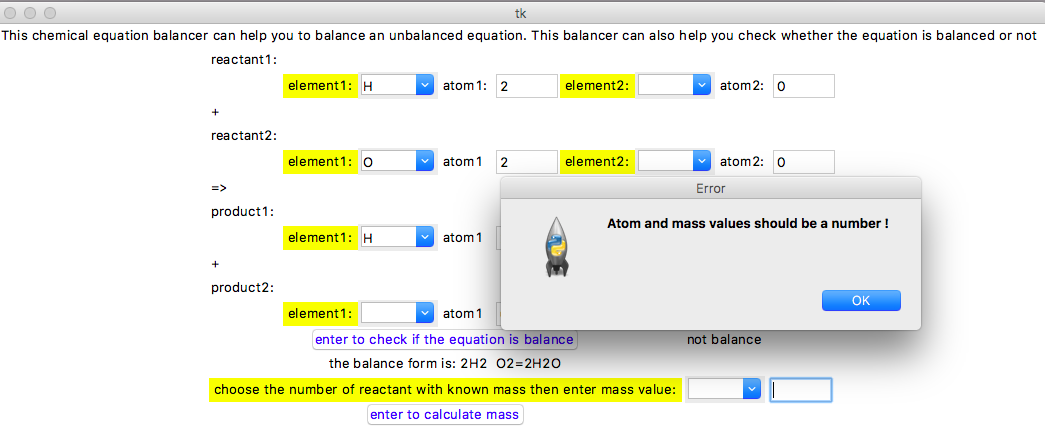
\includegraphics [width=\textwidth]{massnotnumber}
 \caption{\label{ Figure 9:} error massage if user enter non number mass value}
 \end{center}
 \end{figure}
 
\begin{figure}[H]
 \begin{center}
 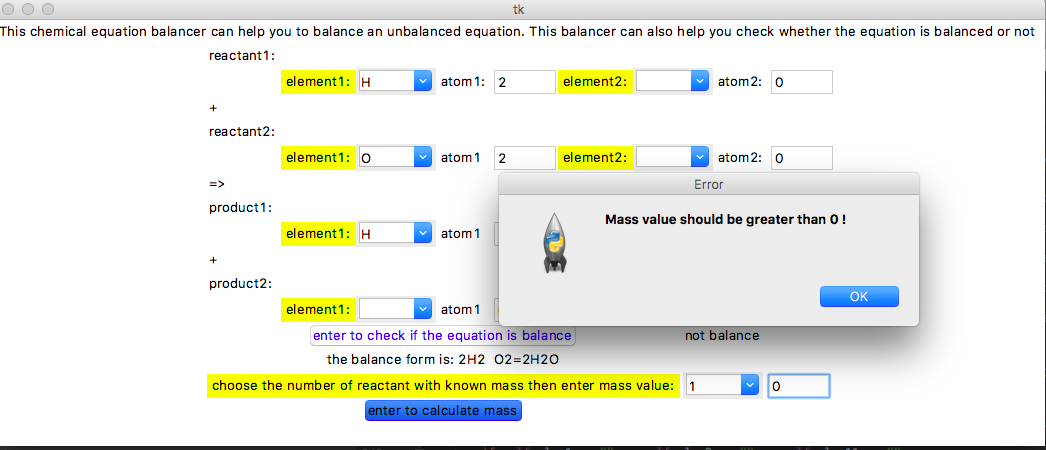
\includegraphics [width=\textwidth]{massnegative}
 \caption{\label{ Figure 10:} error massage if user enter mass less than 1}
 \end{center}
 \end{figure}
 
 
 \subsection{T5: get reactant of known Mass}

The goal of this test is to make sure user select a reactant of a known mass along with entering the mass value before enter the mass calculation button. picture below shows error massage when user did not select a reactant number. The test passed correctly and system responded as intended. 

\begin{figure}[H]
 \begin{center}
 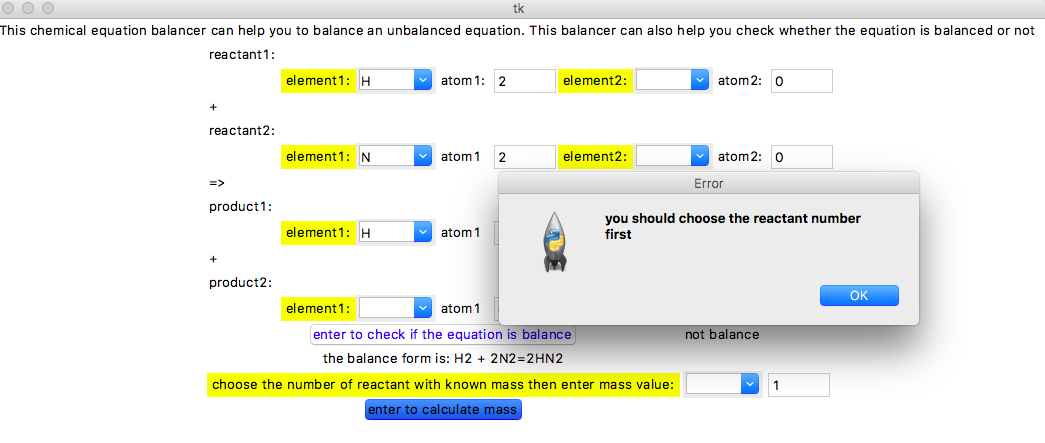
\includegraphics [width=\textwidth]{reactantnumber}
 \caption{\label{ Figure 11:} error massage if user did not select number of reactant with known mass.}
 \end{center}
 \end{figure}

\subsection{T6: Count total number of atoms for each element in each side}

The goal of this test is to make sure that the system count the total of atom values each element involved in the reaction correctly in each side of reaction. add the element name along with the atom total value in dictionary structure to conclude with two dictionaries. one for reactant side and one for product side. picture below shows dictionaries for this reaction: Fe$Cl_3$ + MgO $\rightarrow$ $Fe_2$$O_3$ + Mg$Cl_2$. The test passed correctly and system responded as intended. 


\begin{figure}[H]
 \begin{center}
 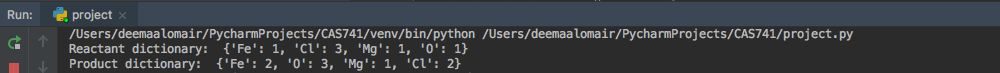
\includegraphics [width=\textwidth]{beforebalance}
 \caption{\label{ Figure 12:} Reactant and Product dictionaries that count the total atoms value for each element}
 \end{center}
 \end{figure}
 
\subsection{T7: Check Balance Test}

The goal of this test is to check if the entered reaction is balance or not. Display "balance" if yes and "not balance" with new balanced form if not. Pictures below shows how system respond to balance and non balance reactions. The test passed correctly and system responded as intended.

\begin{figure}[H]
 \begin{center}
 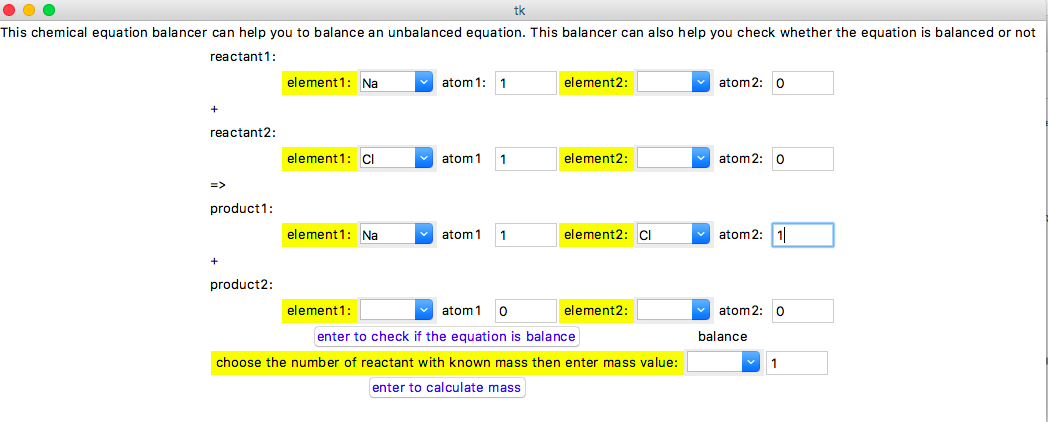
\includegraphics [width=\textwidth]{balance}
 \caption{\label{ Figure 13:} balance reaction}
 \end{center}
 \end{figure}
 
\begin{figure}[H]
 \begin{center}
 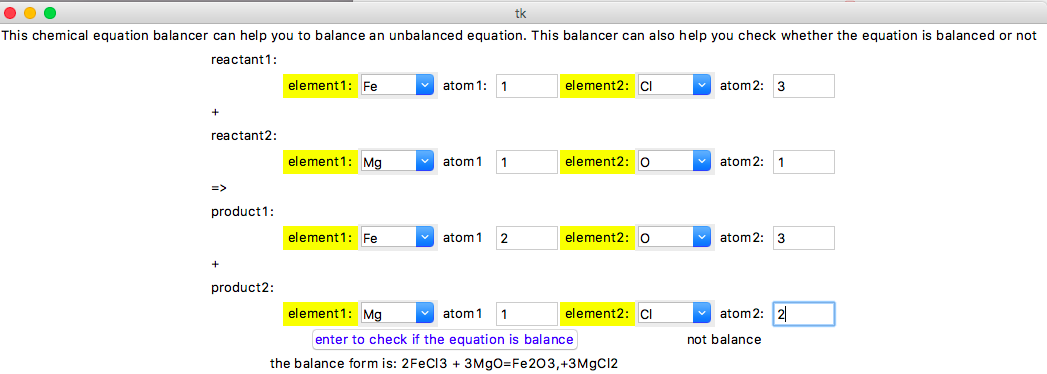
\includegraphics [width=\textwidth]{nonbalance}
 \caption{\label{ Figure 14:} non balance reaction}
 \end{center}
 \end{figure}
  
\subsection{T8: Balance Test}

The goal of this test is to update the created dictionaries: Reactant,Product to make the total atom values for each element in both sides equal. The new dictionaries called : Reactant1, Product1. Picture below shows test passed correctly and system responded as intended.

\begin{figure}[H]
 \begin{center}
 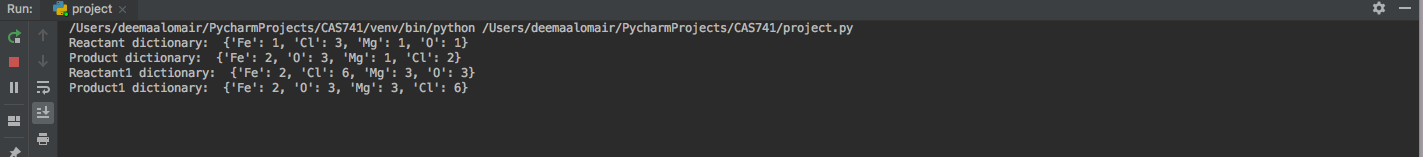
\includegraphics [width=\textwidth]{afterbalancing}
 \caption{\label{ Figure 15:} Reactant1 and Product1 dictionaries after balancing}
 \end{center}
 \end{figure}
 
 \subsection{T9: Coefficients Test}

The goal of this test is to place appropriate coefficients in front of each reactant and product to get the balance form displayed to user . Picture below shows Coefficients values as in test case T9 in \cite{UnitVnVPlan}. test passed correctly and system responded as intended.

\begin{figure}[H]
 \begin{center}
 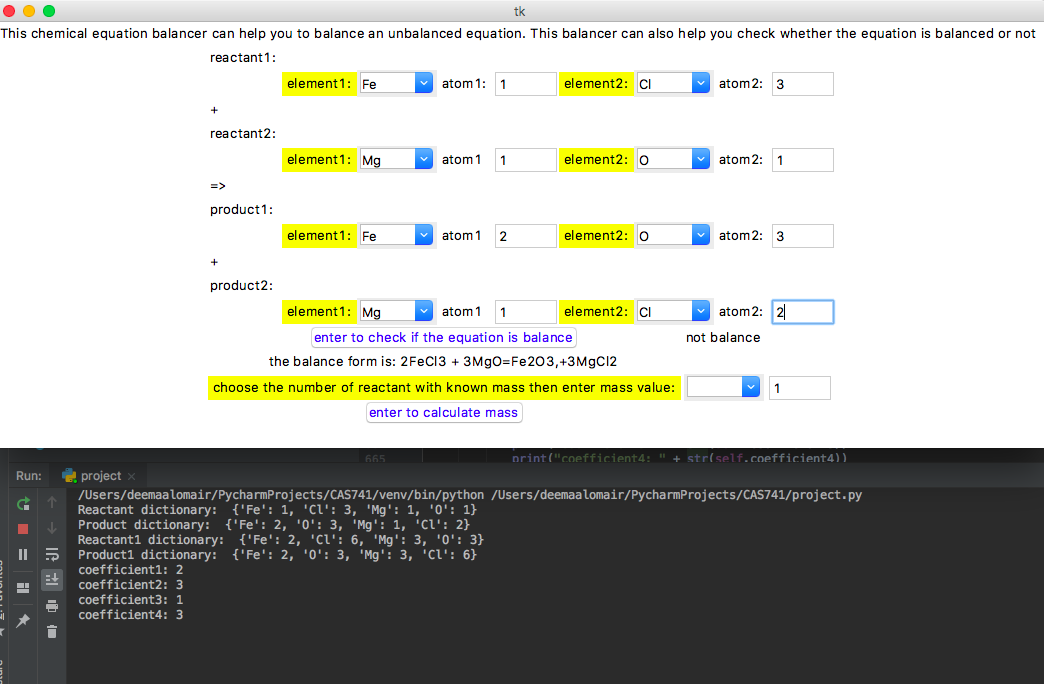
\includegraphics [width=\textwidth]{coff}
 \caption{\label{ Figure 16:} coefficients values}
 \end{center}
 \end{figure}
 
 \subsection{T10: atomic mass Test}

The goal of this test is to get the atomic mass for each element from atomic mass library. Picture below shows atomic mass for element "Fe" and element "O".  test passed correctly and system responded as intended.

\begin{figure}[H]
 \begin{center}
 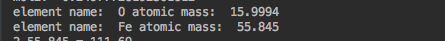
\includegraphics [width=\textwidth]{atomicmass}
 \caption{\label{ Figure 17:} atomic mass value}
 \end{center}
 \end{figure}
 
 \subsection{T11: Molecular Weight Calculation Test}

The goal of this test is to get molecular weight for a reactant. Picture below shows molecular weight is printed for reactant " $Fe_2$$O_3$" as the test case in T10 in \cite{UnitVnVPlan} and the result is identical. Test passed correctly and system responded as intended.

\begin{figure}[H]
 \begin{center}
 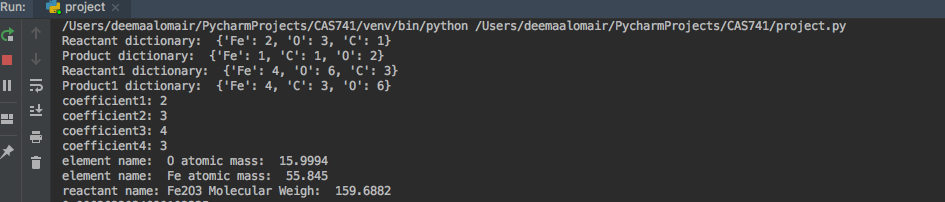
\includegraphics [width=\textwidth]{molecularweight}
 \caption{\label{ Figure 18:} molecular weight value}
 \end{center}
 \end{figure}
 
\subsection{T12: Mole1 Calculation Test}

The goal of this test is to get mole for reactant with known mass. we name this mole "Mole1". Picture below shows Mole1 value printed for reactant " $Fe_2$$O_3$" as the test case in T12 in \cite{UnitVnVPlan} and the result is identical. Test passed correctly and system responded as intended.

\begin{figure}[H]
 \begin{center}
 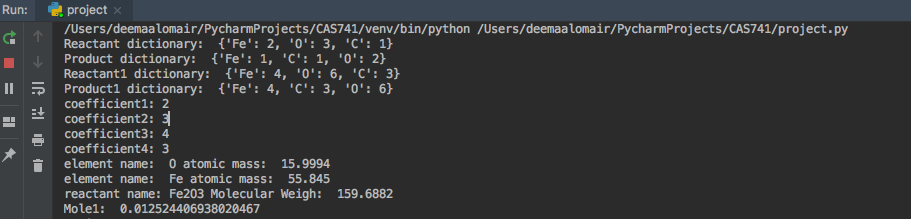
\includegraphics [width=\textwidth]{mole1}
 \caption{\label{ Figure 19:} Mole1 value}
 \end{center}
 \end{figure}

\subsection{T13: Mole Ratio Calculation Test}

The goal of this test is to get mole ratio between given reactants. Picture below shows Mole Ratio value for coefficient of reactant2/coefficient of reactant1 printed  as the test case in T13 in \cite{UnitVnVPlan} and the result is identical. Test passed correctly and system responded as intended.

\begin{figure}[H]
 \begin{center}
 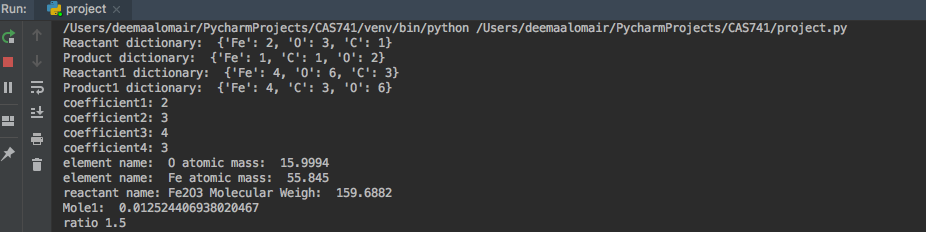
\includegraphics [width=\textwidth]{moleratio}
 \caption{\label{ Figure 20:} Mole Ratio value}
 \end{center}
 \end{figure}

\subsection{T14: Mole2 Calculation Test}

The goal of this test is to get mole for reactant with unknown mass. we name this mole "Mole2". Picture below shows Mole2 value printed as the test case in T14 in \cite{UnitVnVPlan} and the result is identical. Test passed correctly and system responded as intended.

\begin{figure}[H]
 \begin{center}
 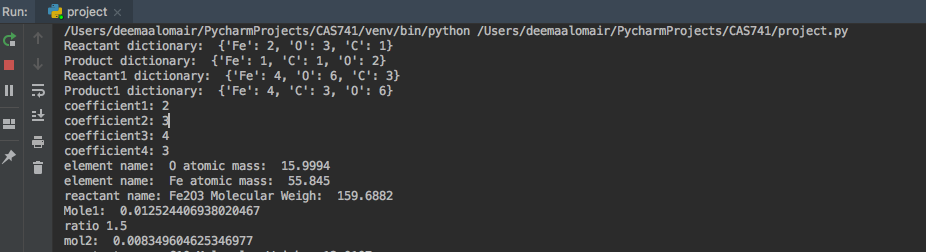
\includegraphics [width=\textwidth]{mole2}
 \caption{\label{ Figure 21:} Mole2 value}
 \end{center}
 \end{figure}
 
\subsection{T15: Mass Calculation Test}

The goal of this test is to get the final mass result for reactant with unknown mass. Picture below shows mass value printed as the test case in T15 in \cite{UnitVnVPlan} and the result is identical. Test passed correctly and system responded as intended.

\begin{figure}[H]
 \begin{center}
 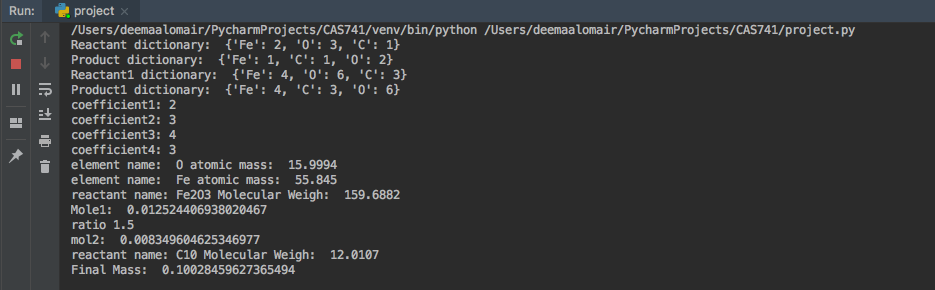
\includegraphics [width=\textwidth]{mass2}
 \caption{\label{ Figure 22:} final mass value}
 \end{center}
 \end{figure}
 
\subsection{T16, T17 : Mass and Reaction Output Test}

The goal of this test is to output the final result including the mass and balance reaction to GUI. This is the main goal of the system. Picture below shows how system will print out the final result to end user. this test is for  test case in T16, T17 in \cite{UnitVnVPlan}. Test passed correctly and system responded as intended.

\begin{figure}[h!]
 \begin{center}
 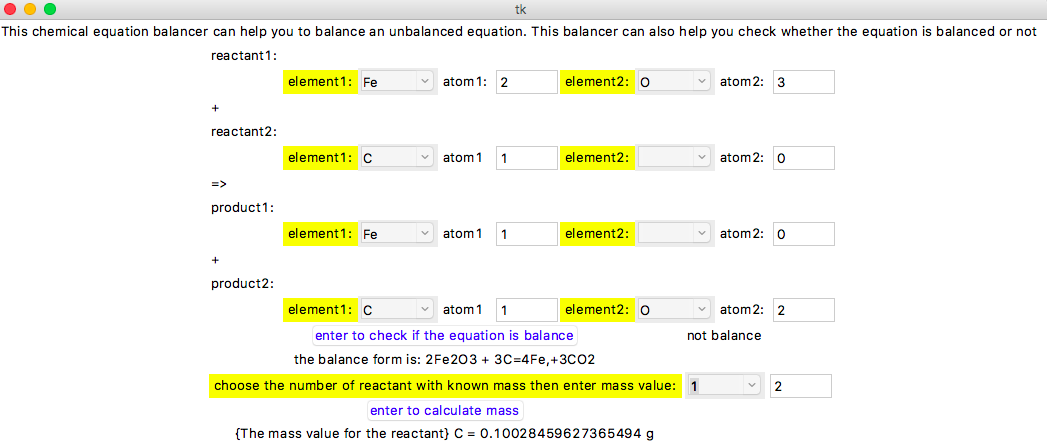
\includegraphics [width=\textwidth]{output}
 \caption{\label{ Figure 22:} final system output}
 \end{center}
 \end{figure}


\section{Changes Due to Testing}
No changes are necessary to the first stage of implementation due to these
test results.

\section{Automated Testing}
\begin{itemize} 
\item coverage testing was preformed using coverage package without any error. blew picture shows coverage testing.
\end{itemize}

\begin{figure}[h!]
 \begin{center}
 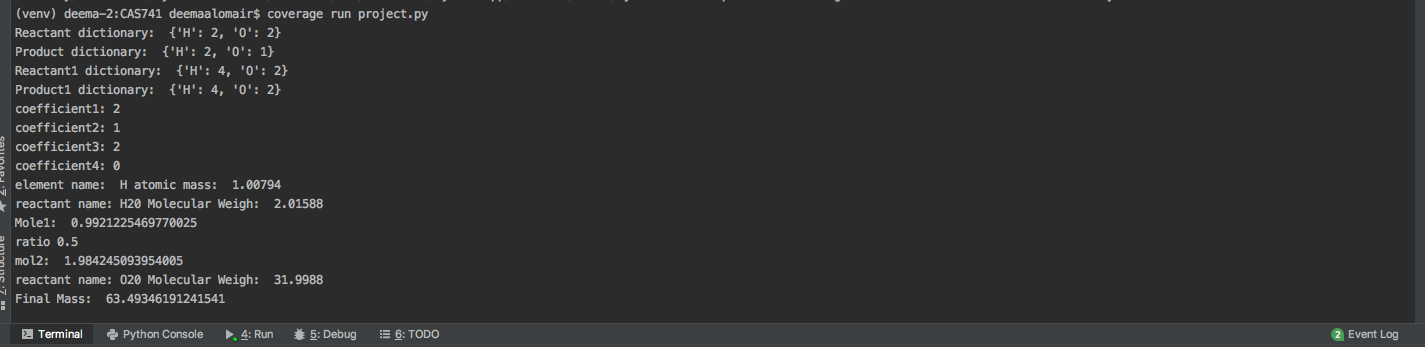
\includegraphics [width=\textwidth]{coverage}
 \caption{\label{ Figure 23:} coverage testing}
 \end{center}
 \end{figure}

		
\section{Trace to Requirements}\label{functional}
\begin{table}[h!]
\centering
\resizebox{\textwidth}{!}{\begin{tabular}{|c|c|c|c|c|c|c|c|c|c|c|c|c|c|c|c|c|c|}
\hline
  & T1 & T2 & T3 & T4 & T5 & T6 & T7 &T8  & T9 & T10 & T11 & T12 &  T13 & T14&T15 & T16 & T17 \\
\hline
R1(input)  & X& X& X& X& X& & & & &  & & & & & & &  \\ \hline
R2(output)  & & & & & & & & & & & & & & & & X & X\\ \hline
R3(calculation) & & & & & &X &X&X & X & X& X& X& X& X& X& &  \\ \hline
R4(VerifyInputOutput)  & X&X &X & X& X& & & & & & & & & & &X &X \\ \hline
\hline
\end{tabular}}
\caption{Traceability Matrix Showing the Connections Between unit test cases and functional requirements}
\label{Table:R_trace}
\end{table}

\begin{table}[h!]
\centering
\begin{tabular}{|c|c|c|}
\hline
  & T18 & T19   \\
\hline
NF1  & & X \\ \hline
NF2  & X& \\ \hline
\hline
\end{tabular}
\caption{Traceability Matrix Showing the Connections Between unit test cases and Nonfunctional requirements}
\label{Table:R_trace1}
\end{table}

\section{Trace to Modules}

A complete description of modules is found in the MG \cite{Designdocument} . A
traceability of unit tests to modules can be found in Table 5 in Section 5.3
of the Unit VnV Plan \cite{UnitVnVPlan}.		

\section{Code Coverage Metrics}
coverage test was done for the whole system and covers all functional requirements. It covers test cases from T1 to T17. 
\newpage
\bibliographystyle{unsrt}

\bibliography{../../refs/References}
\end{document}
